The Deutsch algorithm was originally set up for one qubit by Deutsch in 1985 and then generalized for any number of qubits by Deutsch and Jozsa in 1992 \cite{deutsch1985}. The algorithm has since been improved by R. Cleve et al., which is the version that is discussed here and implemented in the simulation \cite{cleve1998}.

The Deutsch-Jozsa algorithm determines whether a function \( f : \{0,1\}^n \to \{0,1\} \) inside a quantum computer oracle (\(U_f\)) is balanced or constant. If the function is constant, it will return either 0 or 1 for all possible inputs \( \{0,1\}^n\). If the function is balanced, it will return 0 for exactly \( 2^{n-1} \) combinations of \( \{0,1\}^n\) and 1 for the other \(  2^{n-1} \) combinations. The function is promised to be either constant or balanced and nothing else about it is known, it thus serves as a black-box. The internal structure of the function is irrelevant as long as it is either constant or balanced \cite{cleve1998,stolze2008}.

In the worst case, a classical computer would have to evaluate \(2^{n-1}+1\) combinations of \( \{0,1\}^n \) to get a deterministic answer (less for an answer with some uncertainty). The quantum algorithm however only needs a single evaluation to distinguish whether the function is constant or balanced and thus is exponentially faster than a classical computer.

The quantum mechanical function evaluation is implemented as a unitary transformation acting on the quantum register. There are \emph{n} input (control) qubits (the input to the function) and an addition (target) qubit to store the result of the evaluation: \\ \( U_f\ket{ \mathbf{x} , y} = \ket{ \mathbf{x} ,y \oplus f( \mathbf{x} ) }\) \footnote{The \(\oplus\) symbol denotes the exclusive or operation (XOR)} where \( x \in \{0,1\}^n , y  \in \{0,1\} \).

\begin{figure}[H]
	\centering
	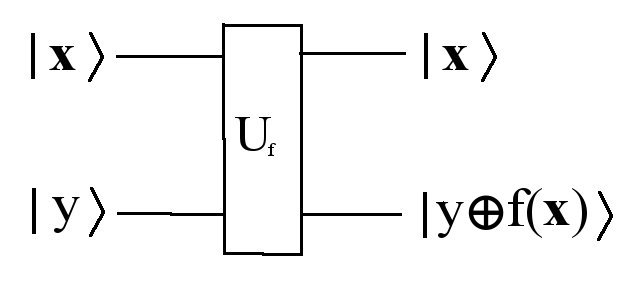
\includegraphics[width=45mm]{./images/deutsch1}
	\caption{Network representation of the oracle.}
\end{figure}

Thus the \emph{n} control qubits stay unchanged and the additional qubit is used to save the result. So for example if \( f(10110) = 1 \) \begin{displaymath} U_f|101101\rangle \to |101100\rangle  \end{displaymath}

\begin{figure}[H]
	\centering
	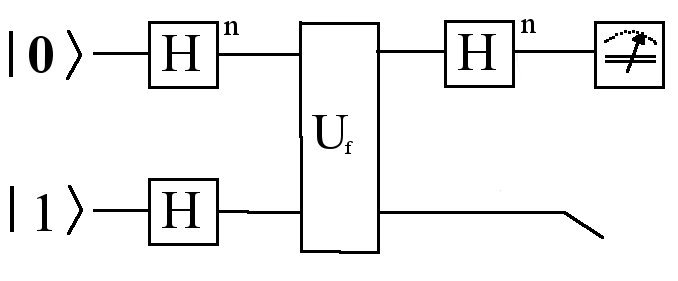
\includegraphics[width=50mm]{./images/deutsch2}
	\caption{Network representation of the Deutsch-Josza algorithm.}
\end{figure}

To run the algorithm, the register is initialized to the state \begin{math} \ket{\mathbf{x},y} = \ket{\mathbf{0},1}\end{math}, so all n control qubits are in state \(\ket{0}\) and the target qubit is in state \(\ket{1}\). A Hadamard gate is then applied to every single qubit causing the new state to be

\begin{equation}
 \frac{1}{\sqrt{2^{n+1}}} \sum_{\mathbf{x} \in \{0,1\}^n} \ket{\mathbf{x}} \otimes (\ket{0} - \ket{1}) 
\end{equation}


After applying the \(U_f\) gate this transforms to

\begin{equation}
 \frac{1}{\sqrt{2^{n+1}}} \sum_{\mathbf{x} \in \{0,1\}^n} (-1)^{f(\mathbf{x})} \ket{\mathbf{x}} \otimes (\ket{0} - \ket{1}) 
\end{equation}

Hadamard gates are then applied to the \emph{n} control qubits, but not to the target qubit, leading to

\begin{equation}
 \frac{1}{2^{n}} \sum_{\mathbf{x},\mathbf{z}\in\{0,1\}^n} (-1)^{f(\mathbf{x})\oplus (\mathbf{x} \cdot \mathbf{z})} |\mathbf{z} \rangle \otimes \frac{\ket{0} - \ket{1}}{\sqrt{2}}
\end{equation}

where \( \mathbf{x} \cdot \mathbf{z} \) is the scalar product modulo two. Now the amplitude of the state \begin{math} |\mathbf{z}\rangle = \ket{\mathbf{0}} \end{math} is 

\begin{equation}
 \sum_{\mathbf{x} \in\{0,1\}^n} \frac{(-1)^{f(\mathbf{x})}}{2^n}
\end{equation}

So if the function is balanced the \( (-1)^{ f( \mathbf{x} ) } \) terms will cancel and the amplitude of \(\ket{\mathbf{0}} = \ket{00...00}\) is zero. If the function is constant the terms will add up to \(\pm1\). Consequently a measurement of the \emph{n} control qubits will yield whether the function in the oracle is constant or balanced. It is constant if the measurement yields 0 and balanced for any other number\cite{cleve1998, stolze2008}.
